\documentclass[margin=0.1in]{standalone}
\usepackage{tikz}
\usepackage{stanli}
\usepackage{amsmath}
\usetikzlibrary{snakes}
\begin{document}

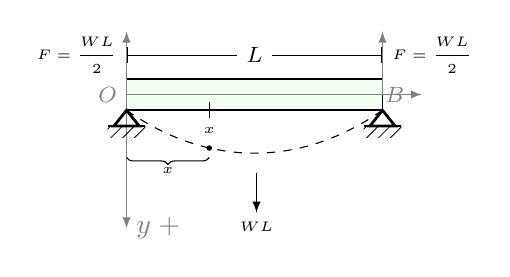
\begin{tikzpicture}[>=latex]
	\filldraw [fill=green!5, semithick] (-0.25,-0.2) rectangle (3,0.2);
	\draw [gray,->] (-0.25,0) node [left] {\footnotesize \(O\)} -- (3.5,0) node [left=1mm] {\footnotesize \(B\)};
	\draw [gray,<->] (-0.25,0.8) --++ (0,-2.5) node [right] {\(y\;+\)};
	\draw [|-|] (-0.25,0.5) node [left] {\tiny \(F= \dfrac{WL}{2}\)} to node [midway,fill=white] {\footnotesize \(L\)} ++(3.25,0) node [right] {\tiny \(F= \dfrac{WL}{2}\)};
	\draw [gray,->] (3,0) --++ (0,0.8);
	\begin{scope}[scale=0.4]
		\point{a}{-0.25}{-0.2};
		\point{b}{3}{-0.2};
		\support{1}{a};
		\support{1}{b};
	\end{scope}
	\def\ang{35}
	\draw [dashed] (a) to [out=-\ang , in=180+\ang] (b);
	\draw (0.8,-0.1) --++ (0,-0.2) node [below] {\tiny \(x\)};
	\fill (0.8,-0.68) circle (1pt);
	\draw [snake = brace, mirror snake] (-0.25,-0.8) to node [midway,below] {\tiny \(x\)} (0.8,-0.8);
	\draw [->] (1.4,-1) --++ (0,-0.5) node [below] {\tiny \(WL\)};
\end{tikzpicture}

\end{document}
